\chapter{MARCO TEÓRICO}

En este capitulo abordaremos los conceptos necesarios que se necesitan para comprender el funcionamiento de un sistema de detección visual, las características del caso de estudio y los diferentes proyectos e investigaciones realizadas sobre la detección de incendios.

Es necesario comprender la manera en que los componentes visuales de los incendios se comportan, el desafío que su detección representa para un sistema informático y realizar un estudio de los métodos y técnicas mas eficaces para su procesamiento y detección.

\section{Definiciones}

\section{Incendios forestales}

Un incendio forestal es la presencia de fuego que consume todo aquello que este cerca y que genere combustión en un terreno forestal. Factores como el tipo de terreno y la velocidad del viento son importantes, y aunque un incendio forestal se genera de manera natural debido a la excesiva acumulación de materia orgánica seca, la mayoría de los incendios forestales son causados por el hombre. El descuido de las personas al visitar zonas forestales abandonando desechos combustibles y actos de vandalismo son los principales factores que influyen en el aumento de riesgo de que ocurra un incendio forestal. 

Los incendios no solo afectan la vegetación, sino también las zonas húmedas debido al aumento de cenizas y polvo, los suelos pierden condiciones de acumulación de agua ocasionando que se degraden fácilmente, se pierde el hábitat de los animales silvestres y se produce la muerte de especies vegetales, animales e incluso vidas humanas.

\section{Detección de incendios forestales}

Esta sección cubre detalles de los elementos visuales que conforman un incendio, el estudio de estos elementos permitió elegir de manera adecuada los métodos y técnicas para su procesamiento y detección.

Una detección temprana de incendios forestales, aumenta la probabilidad de que el combate al mismo sea exitoso y el daño producido sea mínimo. La forma y tamaño de un incendio depende de la temperatura de combustión, la cantidad de suministro de oxígeno y principalmente de los componentes químicos del combustible, es este combustible el que no varia demasiado en áreas forestales y esta principalmente afectado por la época del año ya que esto definirá la velocidad con la cual se realiza la combustión. 

Un incendio forestal, presenta muchas características tales como la temperatura o humedad, pero al tratarse de un sistema visual es necesario centrarse y realizar un estudio de las características visuales del fuego y humo.

\subsection{Características del fuego}

El fuego se produce cuando ocurre la combustión de un elemento inflamable, este desprende una emisión de luz que puede ser muy intensa, el rasgo visual mas característico del fuego es su color, que pueden variar en incendios forestales desde un tono amarillo a naranja.

Aunque en las áreas forestales, no hay objetos naturales con los colores de una llama, es necesario que el sistema pueda distinguir objetos que presenten estos tonos de colores y que sepan diferenciarlos de una llama, para lograr esto es necesario realizar un estudio de otras características de una llama, como los bordes y su variación de color.

\subsection{Características del humo}

El humo se compone principalmente de pequeñas partículas de carbón vegetal completamente quemados y el polvo quemado de modo incompleto. Para los combustibles que normalmente se hallan en áreas forestales, el color del humo se extiende desde un blanco a gris dependiendo de la temperatura del incendio. Si el material está completamente quemado el humo sera semi-transparente y cuando el material esta quemado de forma incompleta, se genera un humo entre semi-transparente a opaco.

Lamentablemente, en áreas forestales se puede presentar objetos que no sean humo y tengan el mismo color, entonces sera asimilado como humo real. Este falso positivo es generado principalmente por objetos que no son humo (nubes, neblina o vapor) con el mismo color que el humo, en este caso, un objeto con el color gris puede causar un falso positivo en la detección de humo. 

Esto hace que el proceso de detección sea complejo y poco fiable. Por tanto, para validar el humo real, además de utilizar su tono de color, se debe tomar en cuenta características del humo tales como su textura, su forma cambiante y la tasa de crecimiento.

\subsection{Desafíos en la detección de incendios}

Durante la detección de incendios forestales, es posible hacer suposiciones de simplificación sobre la apariencia visual del fuego y humo, que a su vez reducen la complejidad del sistema de detección. Estas hipótesis podrían ser que el fuego y humo tienen una determinada tonalidad de color en las áreas forestales, pero dado que un incendio forestal representa un escenario de desastre, no se puede hacer tales suposiciones generales. 

Para detectar con fiabilidad un incendio se deben tomar en cuenta sus siguientes características:

\begin{itemize}
\item El fuego y humo no tienen una forma definida y están en constante movimiento.
\item En áreas forestales, el fuego y humo presentan una gama de colores definida, pero en el ambiente pueden existir otros objetos con colores similares.
\item El humo puede ser fácilmente confundido con neblina, nubes y vapor.
\item Pueden existir objetos que obstaculicen la visión del fuego y humo, que no permitan su correcta detección.
\end{itemize}

Asumimos que, si las condiciones son bastante malas, no va a ser posible que ocurra una detección, independientemente de lo bien que el método de visión por computadora sea usado. Por tanto, una hipótesis de trabajo mínima razonable es que el incendio haya sido captado nítidamente y contenga las características visuales que corresponden a un incendio forestal.

En base a la recopilación de las características y el desafío que representa la detección de incendios, se realiza una descripción de de los métodos y técnicas propuestos para la detección visual de incendios forestales, los mismos serán abordados en la siguiente sección.

\section{Visión por Computador}

Según Haralick (1992), la Visión por Computador es la ciencia que desarrolla las bases teóricas y algorítmicas para obtener información sobre el mundo real a partir de una o varias imágenes \cite{haralick1992robot}, esta es una definición ideal para el caso de estudio que es la detección de incendios, ya que estamos centrados en definir las técnicas y métodos que nos permitan analizar y procesar imágenes, esto con el afán de resaltar sus características y hacerlas únicas con el medio que las rodea.

Para este proyecto de grado este proceso es critico, ya que los resultados obtenidos en la extracción de características son los que serán utilizados en un modelo de entrenamiento que permita realizar una predicción sobre una imagen nueva. 

Esta sección se refiere concretamente a la descripción de los fundamentos teóricos de diferentes técnicas que serán desarrollados durante el proyecto de grado.

\subsection{Tratamiento de imágenes}

Existe muchas funciones para editar imágenes, la mayoría de estas son usadas para optimizar, manipular o retocar las mismas, se usan tres principales funciones para el tratamiento de imágenes. Usando la función de recorte logramos obtener una porción de la imagen que sea de nuestro interés, escalando la imagen lograremos que estas sean del tamaño que deseamos. Es importante tener una cantidad de imágenes de entrenamiento considerable para obtener un mejor modelo de predicción, entonces además de las anteriores se usara una función para reflejar la imagen horizontalmente y una función de rotación, logrando de esta manera obtener una mayor cantidad de imágenes a partir de una sola.

\subsubsection{Recorte}

\paragraph{} El recorte implica la reducción de la imagen, dejando atrás los elementos exteriores para centrar la atención en el tema principal. Dada una imagen de entrada, se establece un tamaño de recorte que queremos obtener (ventana), entonces empezando por la esquina superior izquierda, se obtiene un ``recorte'' de la imagen de entrada del tamaño de la ventana sin afectar la imagen original, recorremos la ventana hacia la derecha unos cuantos pixels y repetimos el proceso hasta llegar al final de la imagen horizontalmente y verticalmente.

\begin{figure}[h!]
\centering
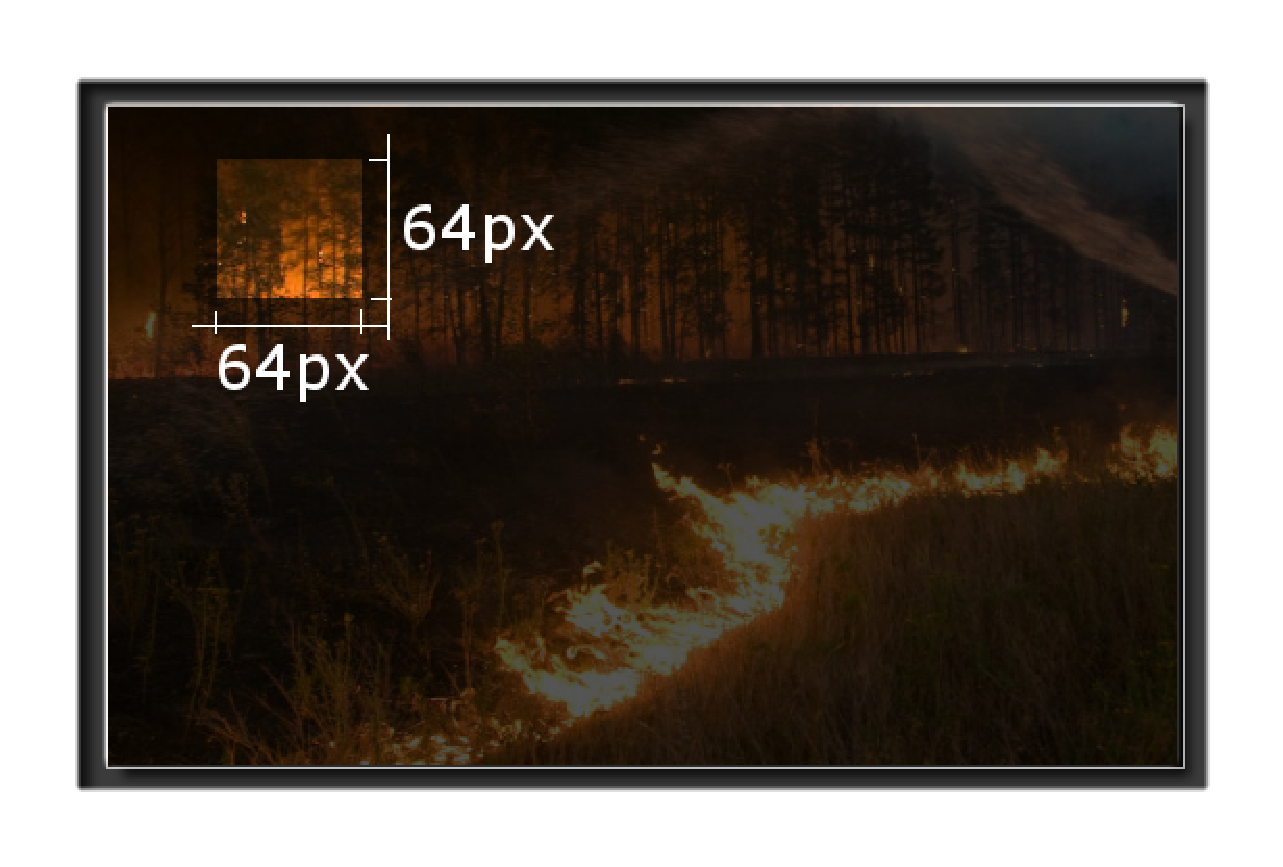
\includegraphics[width=0.5\textwidth , frame]{./imagenes/tratamiento/recorte}
\caption{Sección de la imagen que sera recortada.}
\label{fig:sectorRecorte}
\end{figure}

\paragraph{} Este proceso permite obtener muchas imágenes dada una imagen de entrada que sea de tamaño mayor, entonces solo queda clasificar estas imágenes obtenidas en sus carpetas correspondientes.

\begin{figure}[h!]
\centering
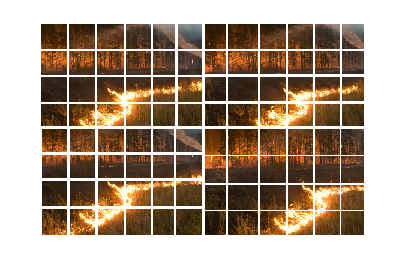
\includegraphics[width=0.5\linewidth , frame]{./imagenes/tratamiento/coleccion}
\caption{Colección de imágenes obtenidas después del recorte.}
\label{fig:coleccion}
\end{figure}

\subsubsection{Puesta en Escala}

\paragraph{} La puesta en escala es la variación del largo y el ancho de una imagen, que en este caso en particular se conservaran las proporciones de la imagen para que esta no quede distorsionada.

\begin{figure}[h!]
\centering
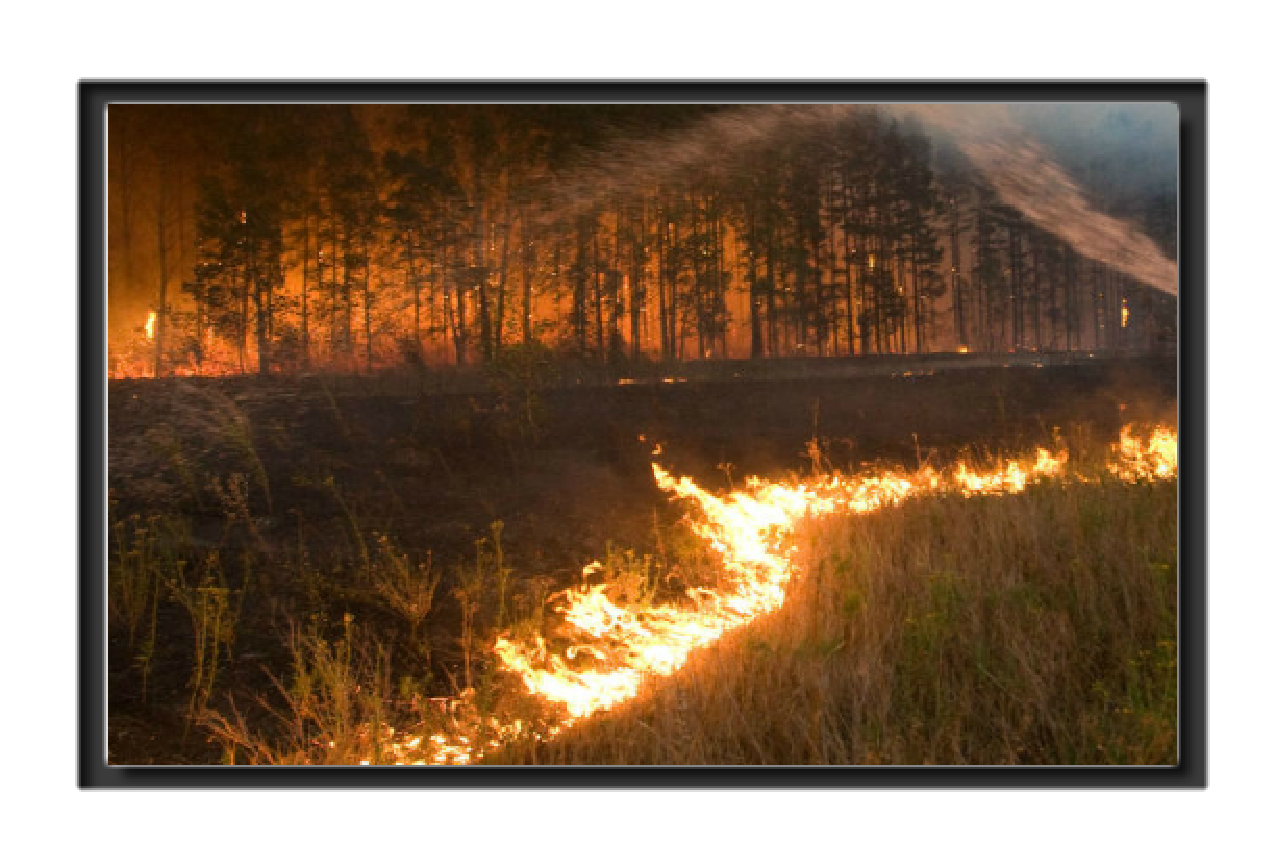
\includegraphics[width=0.6\textwidth , frame]{./imagenes/tratamiento/full_image}
\caption{Imagen original.}
\label{fig:coleccion}
\end{figure}

\paragraph{} Dada una imagen de entrada, modificamos el largo o ancho proporcionalmente hasta obtener el tamaño de imagen que requerimos para nuestro entrenamiento, en caso de que la imagen de entrada no sea perfectamente proporcional al tamaño que deseamos se realizara un recorte de las partes que queden fuera del mismo.

\begin{figure}[h!]
\centering
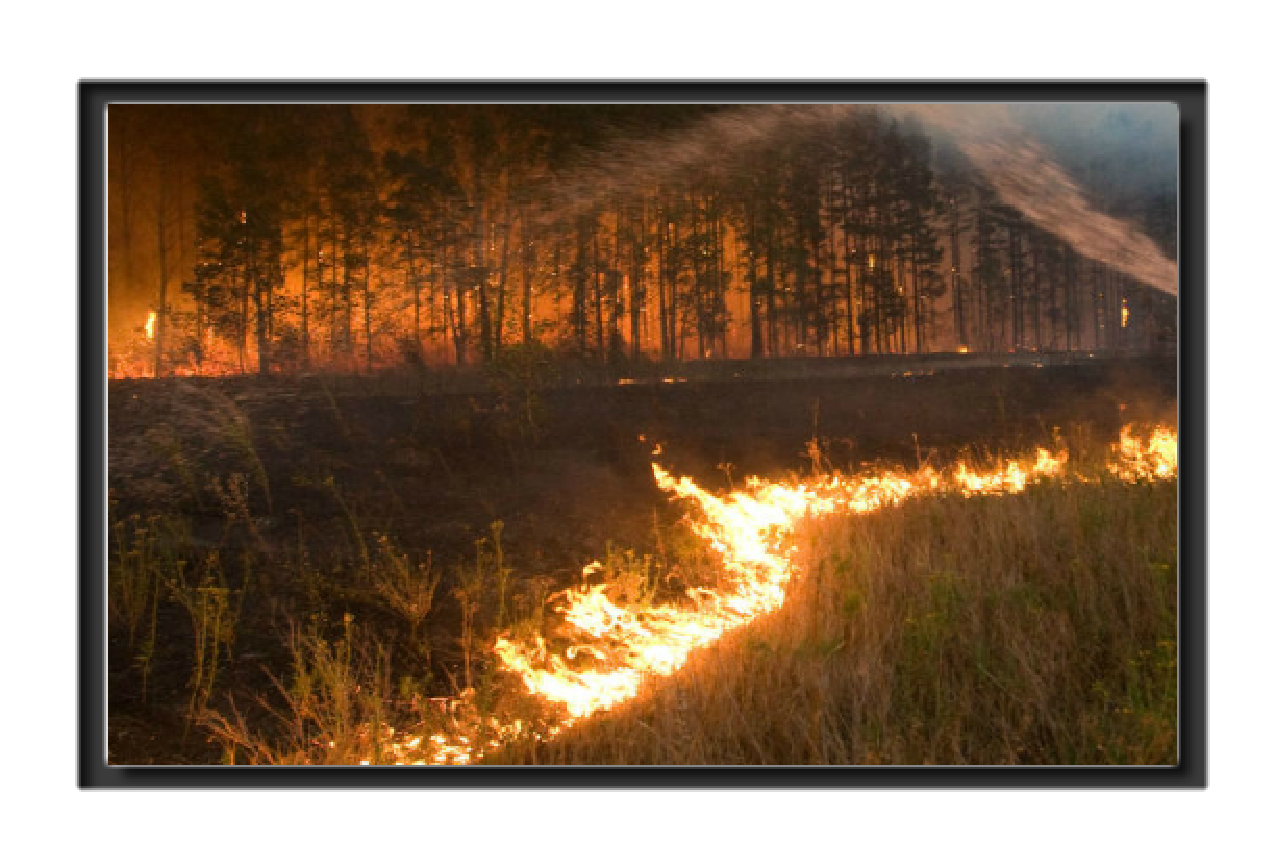
\includegraphics[width=0.3\textwidth , frame]{./imagenes/tratamiento/full_image}
\caption{Imagen después de la puesta en escala.}
\label{fig:coleccion}
\end{figure}

\paragraph{} Con este proceso podemos simular el alejarnos de una imagen o acercarnos a la misma, se debe tomar en cuenta que acercarnos a una imagen ocasionara la perdida de nitidez en el resultado obtenido.

\subsubsection{Refracción }

\paragraph{} Este efecto se logra sometiendo una imagen de entrada a un espejo virtual, entonces la imagen reflejada sera una diferente a la de entrada ya que los pixels de un lado pasaran al lado opuesto.

\begin{figure}[h!]
\centering
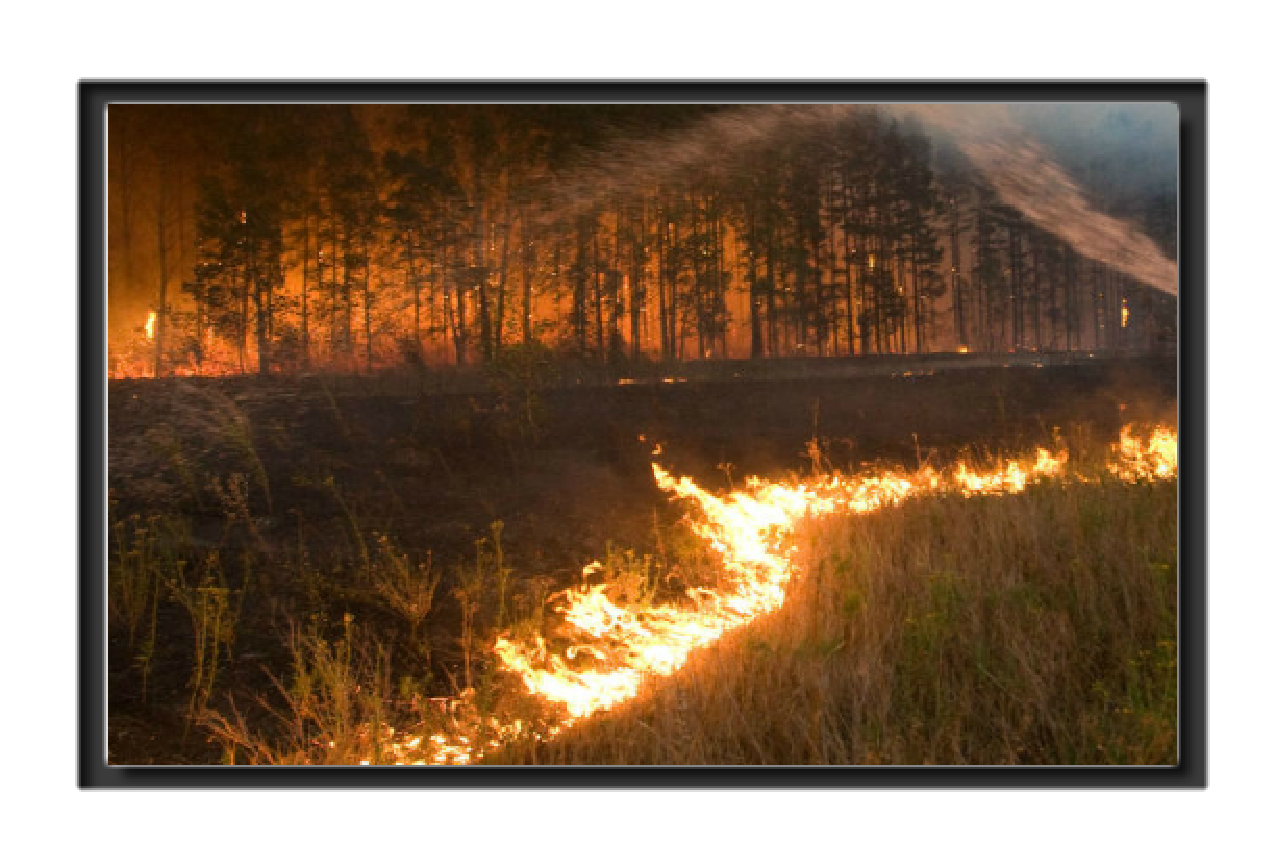
\includegraphics[width=0.5\textwidth , frame]{./imagenes/tratamiento/full_image}
\caption{Imagen original.}
\label{fig:coleccion}
\end{figure}

\begin{figure}[h!]
\centering
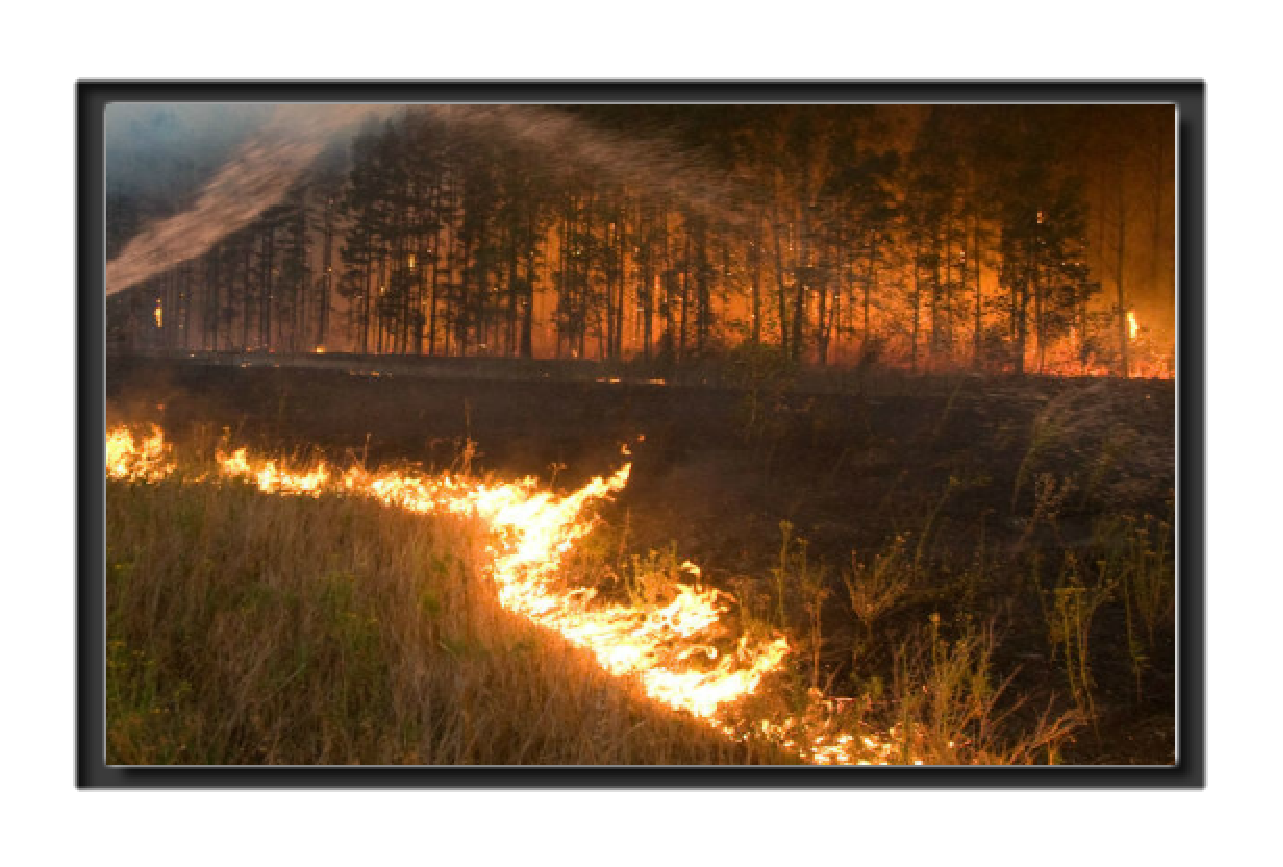
\includegraphics[width=0.5\textwidth , frame]{./imagenes/tratamiento/image_volteada}
\caption{Imagen reflejada.}
\label{fig:coleccion}
\end{figure}


\paragraph{} Dada una imagen de entrada se crea una imagen del mismo tamaño totalmente vacía, y vamos recorriendo la imagen de entrada desde el pixel que esta mas a la izquierda y hacemos una copia del mismo en el pixel que esta mas a la derecha de la imagen nueva. Repitiendo este proceso por toda la imagen de entrada logramos obtener el reflejo en la imagen de salida.

\subsection{Descriptor de características}

\subsubsection{Histogram of Oriented Gradient}

%El año 2005, el concepto de Histograma de Gradientes Orientados fue incluido por N. Dalal y B. Triggs \cite{dalal2005histograms}. Propusieron %un nuevo algoritmo para la detección de personas, que estaba basado en redes de histogramas de gradientes orientados como descriptores de %características, obteniendo de los resultados experimentales que este algoritmo superaba en desempeño a los métodos existentes para la %detección de personas. 

%Es la extracción de características del algoritmo HOG que sera utilizado para el sistema de detección visual de incendios. Este método está %basado en la evaluación de normalizaciones locales de los histogramas de gradientes orientados de una imagen

\subsubsection{Local Binary Patterns}

\section{Aprendizaje Supervisado}

\paragraph{} El aprendizaje automático (Machine Learning) es una rama de la inteligencia artificial cuyo objetivo es desarrollar técnicas que permitan al computador aprender, se trata de crear programas capaces de generalizar comportamientos a partir de una información no estructurada suministrada en forma de ejemplos.

\paragraph{} Uno de los tipos de aprendizaje automático es el aprendizaje supervisado, que se caracteriza por contar con información que especifica qué conjuntos de datos son satisfactorios para el objetivo del aprendizaje. Esto permite reconocer si una imagen dada coincide o no con la imagen que buscamos, para realizar este proceso es necesario cargar al modelo de aprendizaje diferentes imágenes, especificando en el proceso si se trata o no de un incendio.

\paragraph{} Entonces las características obtenidas de una imagen de un incendio mediante técnicas y métodos de Visión por Computador serán las que pasaran al modelo de aprendizaje, además se tiene que realizar el mismo proceso con imágenes que no coincidan con un incendio para enseñarle al modelo que características no pertenecen a un incendio.

\paragraph{} Esta sección describe las diferentes técnicas de aprendizaje supervisado que serán utilizados en el desarrollo de este proyecto de grado.

\subsection{Maquina de Soporte Vectorial}

\subsection{Red Neuronal Artificial}

La Red Neuronal Artificial es una técnica de aprendizaje esta inspirado en el sistema nervioso de los animales, donde grupo de nodos interconectados que representa la red neuronal de un cerebro. Cada nodo representa una neurona artificial y una arista representa la sinápsis que existe entre una neurona y otra siendo el medio de transporte de información de una neurona a otra.

Entonces, la entrada de información se encargara de activar neuronas y si estas son disparadas envían impulsos a otras neuronas a las que está conectada, activando o no las adyacentes entonces este proceso se repetira hasta que finalmente llegue a una neurona de decisión que sera activada o no, determinando si la imagen de entrada es la de un incendio.

\section{Estado del arte}



\section{Resumen del capitulo}

\paragraph{}
En este capítulo se ha proporcionado al lector conceptos que son esenciales para abordar el problema de detección visual de incendios forestales. Debido a las consecuencias medio ambientales que ocasionan los incendios forestales es importante generar herramientas que ayuden su detección temprana para que puedan ser atendidos rápidamente. Mediante la aplicación de técnicas de visión por computadora es posible obtener las principales características que definen el fuego y humo para de esta manera obtener una colección en base a ejemplos de muestra. Es sobre esta colección de características donde se aplica métodos de Aprendizaje Supervisado obteniendo un modelo entrenado capaz de predecir si una imagen presenta fuego o humo en el mismo.

\paragraph{}
La revisión sobre las técnicas de Visión por Computadora, han propuesto varios métodos rápidos y fiables que factiblemente pueden ser implementados en un sistema para la detección de incendios en áreas forestales, el siguiente capítulo describe cómo estos son implementados en el sistema.


